% !TEX root = ../Main.tex
\chapter{含垂直结构的四面体}

下面几类四面体的处理思想都是\textbf{先确定一个面内的外接圆圆心位置}，再过它作该面的垂线找球心。

\section{两侧面是公共斜边的直角三角形}

\state{$\angle APB=\angle AQB=90^\circ$（公共斜边 $AB$）}{
    若四面体里有两个面都是\textbf{以 $AB$ 为斜边的直角三角形}（$P,Q$ 是另两个顶点），则直角 $\angle APB=90^\circ$ 说明 $P$ 在以 $AB$ 为直径的球面上，直角 $\angle AQB=90^\circ$ 说明 $Q$ 也在上面。于是四个顶点都在这个球面上，\textbf{$AB$ 就是外接球的直径}：
    \[
    R=\frac{AB}{2}.
    \]
}

\begin{center}
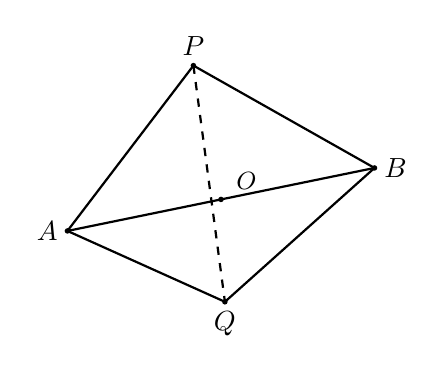
\begin{tikzpicture}[scale=1]
    \coordinate (A) at (-1.8,-0.4);
    \coordinate (B) at (2.1,0.4);
    \coordinate (P) at (-0.2,1.7);
    \coordinate (Q) at (0.2,-1.3);
    \draw[thick] (A)--(P)--(B)--(Q)--cycle;
    \draw[thick] (A)--(B);
    \draw[thick,dashed] (P)--(Q);
    \fill (A) circle (1pt) node[left]{$A$};
    \fill (B) circle (1pt) node[right]{$B$};
    \fill (P) circle (1pt) node[above]{$P$};
    \fill (Q) circle (1pt) node[below]{$Q$};
    \fill (0.15,0) circle (1pt) node[above right,xshift=2pt]{\small $O$};
\end{tikzpicture}
\end{center}

\section{一条侧棱垂直于底面}

\state{$PC\perp$ 平面 $ABC$}{
    若 $PC\perp$ 底面 $\triangle ABC$，则 $PC$ 是\textbf{外接球的一条弦}。球心 $O$ 落在两处的交线上：过 $\triangle ABC$ 外接圆圆心作底面的垂线，再过 $PC$ 中点作 $PC$ 的中垂面。设底面外接圆半径 $r$、$PC=h$：
    \[
    R^2=r^2+\Big(\frac{h}{2}\Big)^2.
    \]
}

\begin{center}
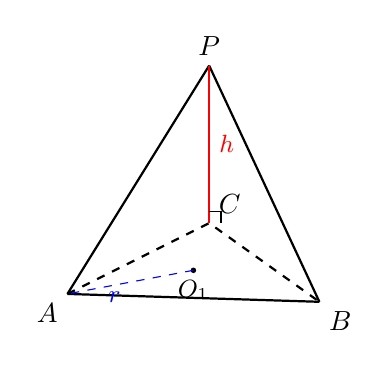
\begin{tikzpicture}[scale=1]
    \coordinate (A) at (-1.6,-0.5);
    \coordinate (B) at (1.6,-0.6);
    \coordinate (C) at (0.2,0.4);
    \coordinate (P) at (0.2,2.4);
    \draw[thick] (A)--(B);
    \draw[thick,dashed] (A)--(C)--(B);
    \draw[thick] (P)--(A) (P)--(B);
    \draw[thick,red] (P)--(C) node[midway,right]{\small $h$};
    \draw[thin] (0.2,0.55)--(0.35,0.55)--(0.35,0.4);
    \coordinate (O1) at (0.0,-0.2);
    \fill (O1) circle (1pt) node[below]{\small $O_1$};
    \draw[dashed,blue] (O1)--(A) node[midway,below left]{\small $r$};
    \node at (P)[above]{$P$};
    \node at (A)[below left]{$A$};
    \node at (B)[below right]{$B$};
    \node at (C)[above right]{$C$};
\end{tikzpicture}
\end{center}

\section{两侧面互相垂直}

\state{平面 $PAC\perp$ 平面 $BAC$（公共边 $AC=l$）}{
    两个面共边 $AC$、互相垂直。设它们的外接圆圆心为 $O_1,O_2$、半径 $r_1,r_2$，$M$ 为 $AC$ 中点。$O_1,O_2$ 到 $AC$ 的距离分别是 $\sqrt{r_1^2-(\frac l2)^2}$、$\sqrt{r_2^2-(\frac l2)^2}$；由两面垂直，这两段互相垂直。球心 $O$ 在 $O_1,O_2$ 上方，于是
    \[
    R^2=\Big[r_1^2-\Big(\tfrac l2\Big)^2\Big]+\Big[r_2^2-\Big(\tfrac l2\Big)^2\Big]+\Big(\tfrac l2\Big)^2
    =r_1^2+r_2^2-\Big(\tfrac l2\Big)^2.
    \]
}

\section{正三角形与直角三角形的组合（二面角）}

有的题把一个正三角形和一个直角三角形\textbf{沿公共边折起}，给出一个二面角。处理的思想还是老一套：在两个面里各定出外接圆圆心 $O_1,O_2$，过它们作各自面的垂线，球心 $O$ 在两条垂线的交点处；二面角决定了两条垂线的夹角，把 $OO_1$、$OO_2$ 与两段到公共边的距离放进同一个空间直角三角形里解出 $R$。这类题没有现成公式，靠的是\textbf{把球心拆到两个面上去}这一招。
